\section{Theoretische Grundlagen}
\label{sec:theorie}

\subsection{Entstehung und Zerfall kosmischer Myonen}

Treffen Protonen kosmischer Höhenstrahlung auf die Moleküle der Luft, entstehen unter anderem Pionen und Kaonen, die daraufhin einen hadronischen Teilchenschauer auslösen können. \\
Die hier betrachteten kosmischen Myonen sind ein Teil dieses Luftschauers, der direkt aus den Pion- und Kaonzerfällen entsteht. \\

Unter Erzeugung eines Myons und Myonneutrinos zerfallen diese wie folgt:

\begin{align*}
    \pi^- &\rightarrow \mu^- + \bar{\nu}_\mu \\
    \pi^+ &\rightarrow \mu^+ + \nu_\mu \\
    K^+ &\rightarrow \mu^+ + \nu_\mu \,.
\end{align*}

Die in etwa $10 - 15 \,\unit{\kilo\meter}$ \cite{grup} entstehenden Myonen besitzen die selben Eigenschaften wie Elektronen, mit dem Unterschied, dass Myonen etwa die 200-fache Masse \cite{pdg} besitzen .
Auch mit einer Lebensdauer von etwa $2,187 \cdot 10^{-6} \,\unit{\second}$ \cite{pdg} erreicht aufgrund der hochrelativistischen Geschwindigkeiten etwa 
$1 \,\text{Myon} \, (\unit{\centi\meter}^2 \, \unit{\minute})^{-1}$ die Erdoberfläche \cite{grup}. \\

Erreicht ein Myon das Ende seiner Lebensdauer, zerfällt es unter Austausch eines W-Bosons über den folgenden Kanal:

\begin{equation*}
    \mu \rightarrow e + \nu_e + \nu_\mu \,,
\end{equation*}

wobei immer ein Neutrino und ein Antineutrino so entsteht, dass die Leptonzahl erhalten bleibt. \\
Für positive Myonen ist dieser Zerfall der einzig mögliche, negative Myonen können dagegen auch durch Myoneinfang zerfallen.
Dabei wird das wie ein Elektron negativ geladene Myon von einem Atomkern angezogen und löst aufgrund seiner gegenüber Elektronen größeren Masse eine Elektronenkaskade aus,
bis es auf das niedrigste Energieniveau fällt und vom Kern unter Entstehung eines Neutrons und eines Neutrinos eingefangen wird:

\begin{equation*}
    \mu^- + p \rightarrow n + \nu_\mu \,.
\end{equation*}

Dadurch erhält das negative Myon genau genommen eine geringere Lebensdauer.


\subsection{Berechnung der Lebensdauer}

Zur Berechnung der Lebensdauer wird im Folgenden von einem exponentiellen Zusammenhang der Form
\begin{equation}
    N(t) = N_0 \, e^{-\lambda \, t}
    \label{eq:expdec}
\end{equation}
zwischen der Anzahl der Myonen zum Zeitpunkt $t_0 = 0$ und der Zeit $t$ ausgegangen. 
Dabei bezeichnet $N_0$ die Anzahl der Myonen zu Beginn, $N(t)$ die Anzahl nach einer Zeit $t$ und $\lambda$ die charakteristische Zerfallskonstante des Prozesses. \\

Die Lebensdauer $\tau$ lässt sich mit dem zeitlichen Erwartungswert $<t>$ identifizieren.
Es gilt
\begin{equation}
    \tau = <t> = \int_0^\infty \text{d} t \, \lambda \, t \, e^{-\lambda \, t} = \frac{1}{\lambda} \,.
\end{equation} 

Für diesen Versuch muss \eqref{eq:expdec} um einen Untergrund $B$ ergänzt werden, um alle gezählten Ereignisse zu beschreiben, sodass
\begin{equation}
    N(t) = N_0 \, e^{-\lambda \, t} + B
    \label{eq:exponential_decay}
\end{equation}
gilt.

Zur Abschätzung dieses Hintergrundes treffe innerhalb einer Suchzeit $T_\text{s}$ nach Eintreffen des ersten Myons ein weiteres als unerwünschter Untergrund ein.
Für die durchschnittliche Anzahl gemessener Myonen pro Sekunde während der gesamten Messzeit $T_\text{mess}$ gilt
\begin{equation*}
    n = \frac{N_\text{start}}{T_\text{mess}} \,,
\end{equation*}
wobei $N_\text{start}$ die Anzahl der gegebenen Startsignale, also die Anzahl der eintreffenden ersten Myonen beschreibt. \\

Das Produkt $T_\text{s} \cdot n$ beschreibt den Erwartungswert der Messungen in der Suchzeit. \\

Damit lässt die poissonverteilte Wahrscheinlichkeit für das Eintreffen $k$ weiterer Myonen durch
\begin{equation*}
    P(k) = \frac{(T_\text{s} \cdot n)^k}{k!} \, e^{T_\text{s} \cdot n}
\end{equation*}
beschreiben. \\

Über
\begin{equation*}
    N_\text{fehl} (k) = N_\text{start} \cdot P(k)
\end{equation*}
lässt sich so die Anzahl der Fehlereignisse berechnen, wobei hier insbesondere $P(1)$ wichtig ist. \\
Mit $P(1)$ ergibt sich
\begin{equation}
    N_\text{fehl} (k) =  {N_\text{start}}²  \cdot \frac{T_\text{s}}{T_\text{mess}} \, e^{{ N_\text{start}} \cdot \frac{T_\text{s}}{T_\text{mess}}}
    \label{eq:theo_unter}
\end{equation}


\newpage

\subsection{Erklärung wichtiger Bauelemente}

Die Erklärung der im Versuch verwendeten Bauelemente erfolgt nach \autoref{fig:schaltung}.

\begin{figure}[H]
    \centering
    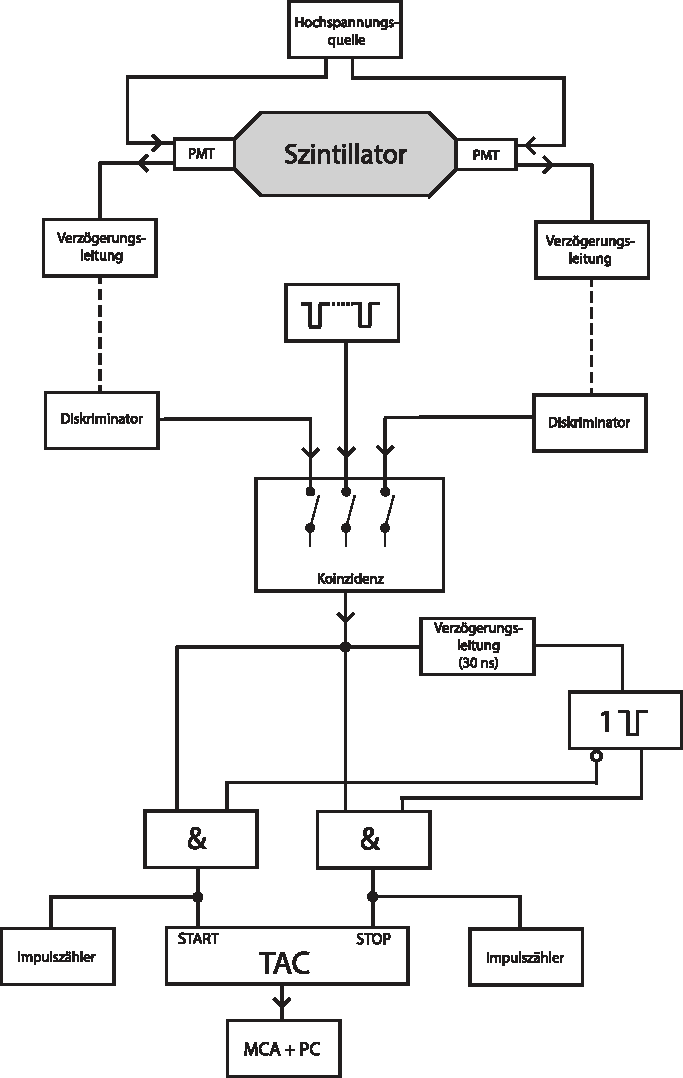
\includegraphics[width=.6\textwidth]{figures/V01.pdf}
    \caption{Schaltbild der verwendeten Messelektronik \cite{ap03}.}
    \label{fig:schaltung}
\end{figure}

\subsubsection{Szintillator}

Bei dem ersten verwendeten Bauteil handelt es sich um einen flüssigen organischen Szintillator. Der Unterschied zu anorganischen Szintillatoren besteht darin, dass hier nicht das Szintillatormaterial
ionisiert wird und sich ein Elektron zum Aktivierungszentrum bewegen muss, um ein Photon auszulösen, sondern dass das Szintillatormaterial auf ein höheres Energieniveau angeregt wird.
Diese Anregungsenergie wird innerhalb einiger Nanosekunden wieder freigesetzt \cite{kolawerm}. \\
Die Zeitauflösung organischer Szintillatoren ist deutlich höher als die anorganischer Szintillatoren.
Aufgrund der Vielfalt unterschiedlicher Anregungsniveaus organischer Szintillatoren ist die Energieauflösung verglichen mit den diskreten Ionisationsenergien der anorganischen Szintillatoren geringer.
Für Lebensdauermessung ist besonders die Zeitauflösung wichtig, also eignen sich organische Szintillatoren am besten. \\


\subsubsection{Photomultiplier}

Der Photomultiplier (PMT) wandelt mithilfe des Photoeffekts ein eintreffendes Photon in ein elektrisches Signal um.
Über eine anliegende Beschleunigungsspannung wird das vom Photon ausgelöste Elektron zur Anode beschleunigt und löst auf seinem Weg weitere Elektronen aus.
An der Anode lassen sich diese Elektronen als Strom messen.
Insgesamt wird das vom Szintillator eintreffende Signal um einen Faktor von bis zu $10^9$, für gewöhnlich um $10^5 - 10^7$-fach, verstärkt \cite{kolawerm}.


\subsubsection{Verzögerungsleitung}

In den Verzögerungsleitungen liegen Leitungen unterschiedlicher Länge, sodass das eintreffende Signal mit Schaltern über die Leitungen umgeleitet werden kann.
Das Signal legt eine längere Strecke zurück und ist damit verzögert. Die hier verwendeten Verzögerungsleitungen verfügen über sieben unterschiedliche Schalter, mit denen Einzelverzögerung
zwischen $1 \,\unit{\nano\second}$ und $32 \,\unit{\nano\second}$ eingestellt werden können. Diese Schalter funktionieren additiv.


\subsubsection{Diskriminator}

Die verbauten Diskriminatoren verfügen über eine regelbare Schwellamplitude. Alle eintreffende Impulse unter dieser Amplitude werden nicht weitergegeben, sodass unerwünschte Störsignale,
die beispielsweise durch zufällig ausgelöste Elektronen im PMT entstehen, unterdrückt.


\subsubsection{Koinzidenz}

Die Koinzidenz liefert nur dann einen Output, wenn an allen Eingängen gleichzeitig ein Eingangssignal eintrifft.


\subsubsection{Monostabile Kippstufe}

Die monostabile Kippstufe, auch Monoflop genannt, besitzt zwei unterschiedliche Zustände. Trifft ein Impuls am Monoflop ein, wird dieser von seinem Grundzustand in den angeregten Zustand geschaltet,
in dem er für eine definierbare Zeit verbleibt, bevor er sich wieder umschaltet. Dabei gibt er in beiden Positionen ein Signal aus.


\subsubsection{Time-Amplitude-Converter}

Der Time-Amplitude-Converter (TAC) verfügt über zwei Eingänge. Treffen zwei Signale nicht gleichzeitig ein, gibt er ein Ausgangssignal, dessen Amplitude proportional zum zeitlichen Abstand der beiden
Eingangssignale ist.


\subsubsection{Vielkanalanalysator}

Der Vielkanalanalysator (engl. Multichannel Analyser [kurz MCA]) sortiert Eingangssignale nach ihrer Amplitude in unterschiedliche Kanäle, erstellt also ein Histogramm der Eingangsdaten.





